\section{Discussion}\label{disc}
%What 'advice' to give to the reader? Discuss difficulties (e.g. tosca) and such.

% include preliminary performance measurements, emphasize that it's outside the scope of our research, no real conclusions should be made, just observations, this needs to be made very clear

%Metadata, rules, web resolver link or not etc. all depending on PID and cloud proivider.


%%% ZHAO feedback
    %   - how do they work as a whole
    %   - Demonstrate its usage via example: show all components
    %   - some performance study etc?
    %   - summarize what you did
    %   - novelty (quality of being new and original)
    %   - weakness



%Discussion or future work.
For our proof of concept we created two scripts for the client side and two scripts for the gateway to demonstrate our design. The gateway and client are conceptually part of the NDN network we have setup with Kubernetes and can be scaled in or out. The responsibility of the scripts on the client side is to retrieve a requested object either from the PID server or from NDN. The scripts that are implemented in the gateway send either the PID link or the name in NDN to the client for retrieval of the requested object after translation. This depends on the object being published in NDN or not.

To cache a object in NDN in our proof of concept, the user is required to first request the object from the PID server. The object can be requested in NDN afterwards. Therefore,  transparency has not been implemented, but can be achieved. In previous studies, user input was required after translation, which is also the case in our current proof of concept. In section \ref{pid-poc} we describe how transparency can be achieved by combining the scripts that we have created by adding a statement. This statements checks whether a object is already published in NDN.

%Usually, NDN operates with in-network caching. However, we used \texttt{ndnputchunks} to cache objects in NDN in our proof of concept, which does not serve a file but works with a standard input stream. Data is cached in-memory and takes up to three times the size of the object for encoding \cite{ndnput-mem}. For using a persistent file cache we already compiled the base image of our proof of concept with repo-ng\footnote{https://github.com/named-data/repo-ng} as that utilizes
%is part 
%the NDN-CXX application we already use. Repo-ng is an open source project and is used to set up a data repository for a persistent file cache.

For supporting multiple PID types, we demonstrated the use of three PID types in our proof of concept. This already proves that supporting multiple PID types is possible. Adding more PID types to our proof of concept, such as the ones described in Karakannas' research \cite{icn-bd} is possible but we see this more as work for an implementation.

%TCP PID part still has to be adjusted to new PID server. 
%> Done
%"NDN is not designed for retrieving data objects with big sizes", as Zhao stated. 
%It is meant for "large datasets" (which could be a lot of small files) and not "large objects". 
%Maybe that's why we don't see that much of a difference between NDN vs TCP/IP for a 1000MB object in comparison to NDN vs TCP/IP for a 100MB object... 
%Should we also state this and remove the 1000MB benchmark and run some benchmarks with a 10MB file? 
%> Done
%First time is not taken into account. So results are based on direct link between consumer and router where the data is cached.

In figure \ref{fig:perftest-1} and \ref{fig:perftest-2} preliminary performance results are shown of our PID server and the NDN network we setup. We ran the performance tests within our proof of concept and used a 10MB and 100MB data object, to demonstrate the performance of retrieving a small and a large data object. We can observe that NDN over UDP outperforms the TCP/IP connection used for retrieving data objects from the Handle PID server that we setup. In turn, NDN over TCP outperforms NDN over UDP. This result correlates with the work done by Lim et al. \cite{lim2018ndn}. Their research concludes that NDN provided performance improvements compared to classical climate data delivery techniques based on TCP/IP. In addition to this, NDN over TCP demonstrated a more reliable and faster performance due to the allowance of larger dynamic window sizes and congestion control.

\begin{figure}[H]
\centering
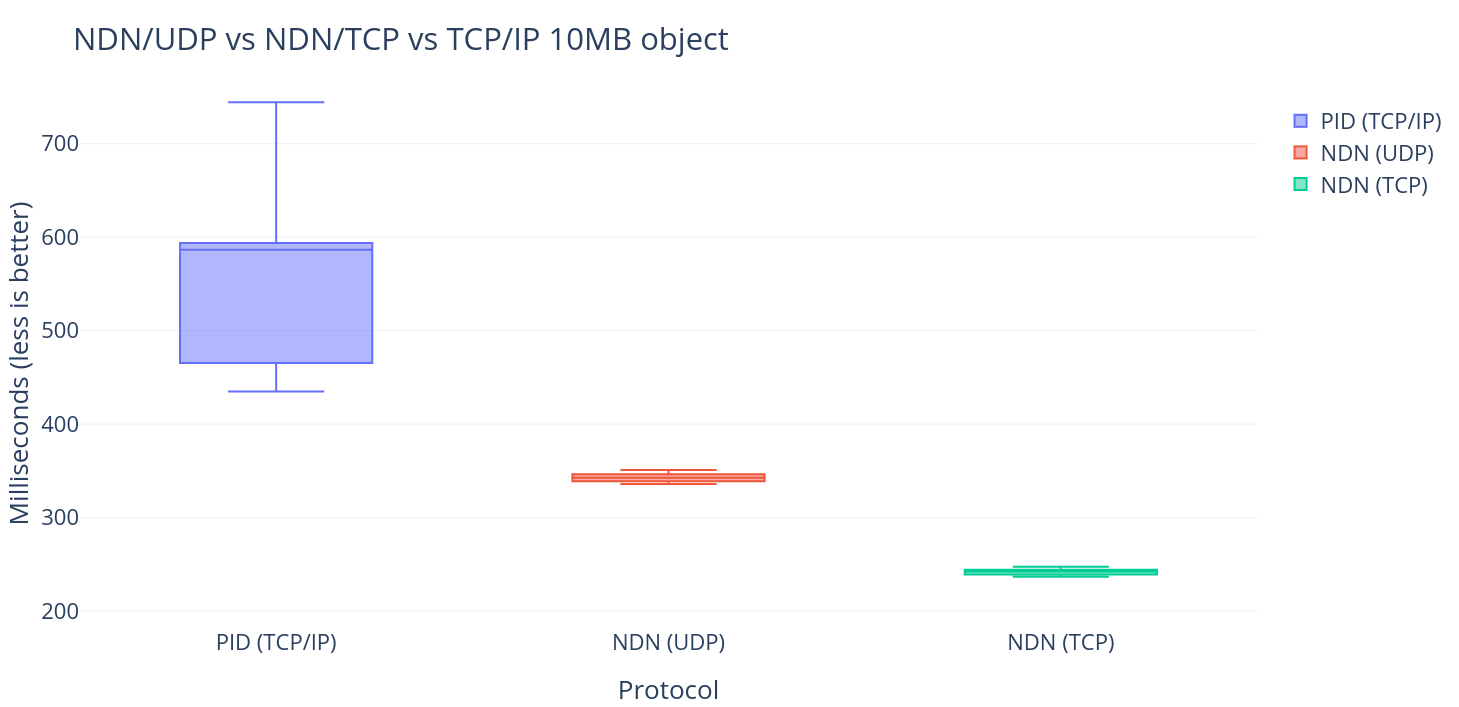
\includegraphics[scale=0.3]{Images/bench10MB.png}
\caption{Performance test TCP/IP vs NDN with a 10MB object.}
\label{fig:perftest-1}
\end{figure}

\begin{figure}[H]
\centering
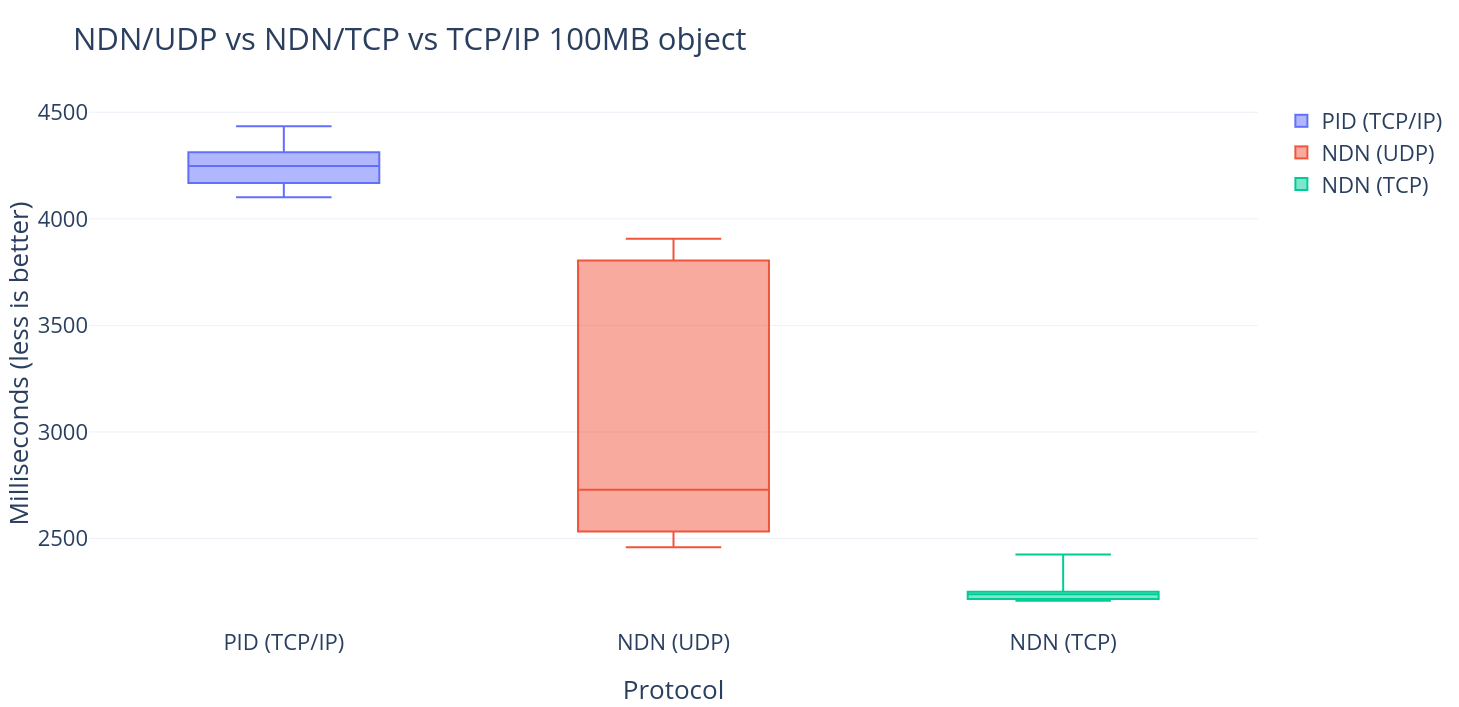
\includegraphics[scale=0.3]{Images/bench100MB.png}
\caption{Performance test TCP/IP vs NDN with a 100MB object.}
\label{fig:perftest-2}
\end{figure}

We want to highlight that the results we present in figure \ref{fig:perftest-1} and \ref{fig:perftest-2} are preliminary. A range of parameters can be optimized within NDN, this is highlighted in section \ref{fut}, where we discuss benchmarking NDN in more detail.


TO-DO: 
- Mention TOSCA difficulties.
- Preliminary benchmark results (PID server on nimes)
% high-availability kubernetes + persistent volumes + ndn cache